

\subsection{Introduction}
Our S\&C subsystem consists of a 
\begin{itemize}
    \item Control Boards: \begin{itemize}
            \item Braking Controller
            \item Thermal (Cooling) Controller
    \end{itemize}

    \item Telemetry Device: \begin{itemize}
            \item CAN Bus
            \item Telemetry Transceiver
            \item Network Transceiver
            \item GUI/Logging system
    \end{itemize}

\end{itemize}

\subsubsection{FDD.9 Budget, Funding, and Manufacturing Methods}
Due to our sponsoring agreements with Mouser, Wurth and . We were able to receive
 
\subsection{Technical Description and Constraints}
\subsubsection{FDD.11 Technical Specifications}
All sensors 

The software follow a simple state: \\
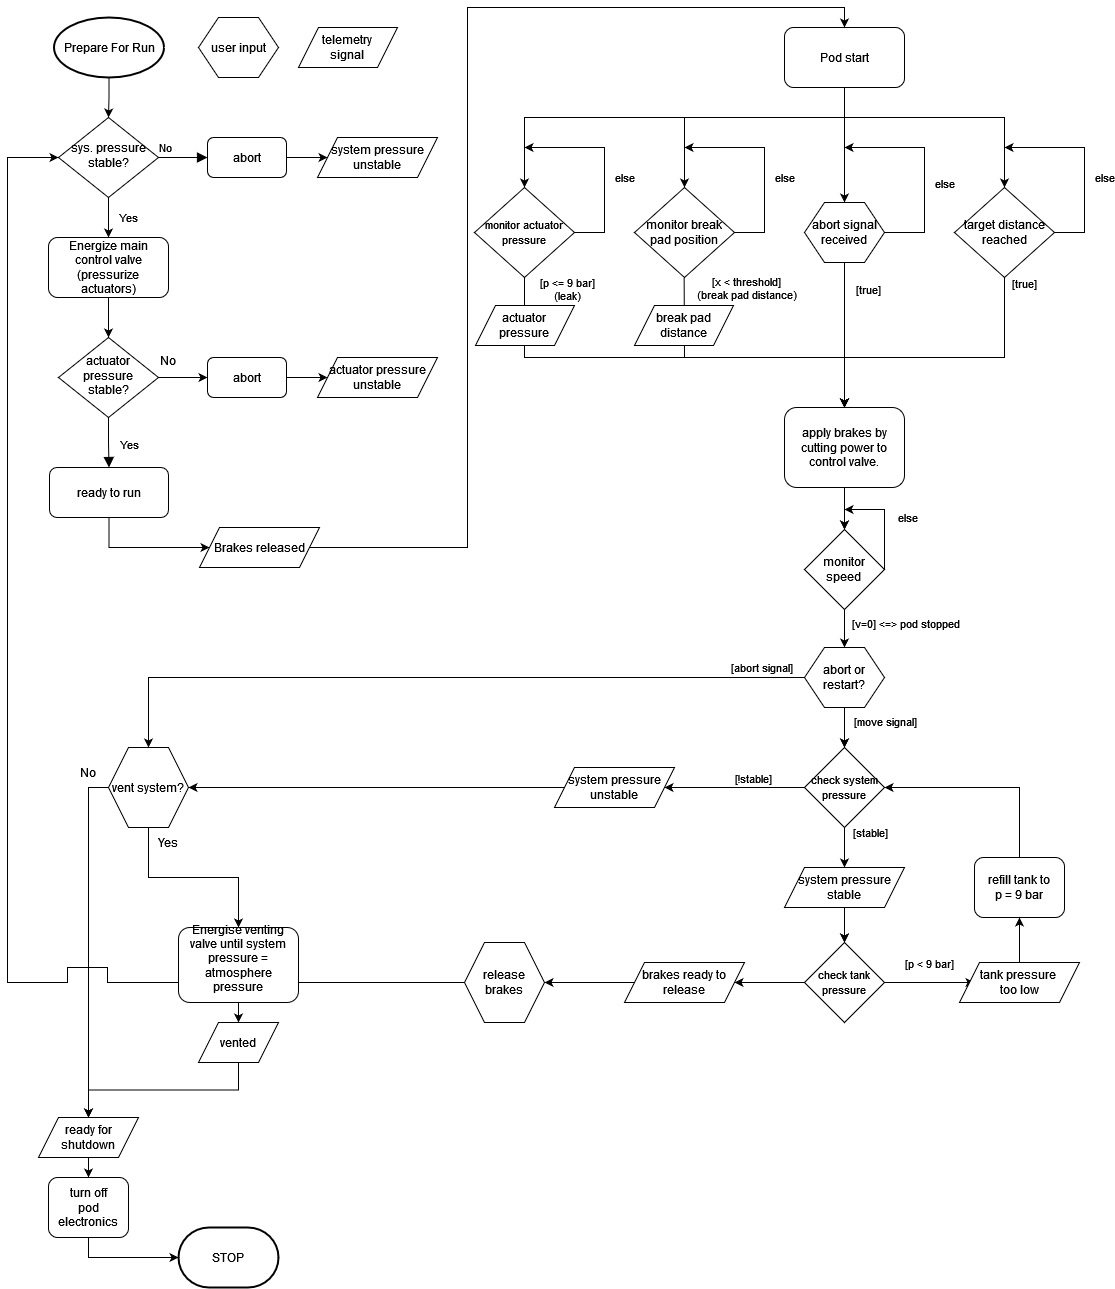
\includegraphics[width=\textwidth]{texfiles/elec/eimg/brakesoftware_ext}
 
\subsubsection{FDD.17 Design Constraints}
The
 
\subsubsection{FDD.18 Performance Requirements}
We designed with a failure-proof 
 
\subsubsection{FDD.19 Integration with Other Systems}
The friction brakes, the cooling pump and the motor are controlled through our system.
 
\subsection{Objectives and Design Approach}
\subsubsection{FDD.12 Design Objectives}
 
\subsubsection{FDD.15 Innovative Aspects}
\par We are able to measure the vibrations of our chassis in different places, proving our mechanical simulations.
\subsubsection{FDD.16 Design Approach}
 
\subsection{Safety}
\subsubsection{FDD.13 Safety Considerations}
 
\subsubsection{FDD.14 Safety Testing and Compliance}
 
\subsection{Parts List (FDD.21)}
% Comprehensive list of all parts used in the braking system, including specifications and suppliers.
Parts list:
\begin{table}[h]
    \centering
    \caption{Parts List}
        \begin{adjustbox}{width=\textwidth,center}
    \begin{tabular}{|c|c|c|c|c|c|c|}
        \hline
        \textbf{Amount} & \textbf{Name} & \textbf{Company, (Serial Number)} & \textbf{Dimensions [mm x mm x mm]} & \textbf{Weight [kg]} & \textbf{Nominal Voltage} & \textbf{Expected max current} \\
        \hline
        32 & Additional Temperature Sensors (NTC, 10k Ohm) & Company & 2x2x2 & 0 & - & - \\
    \end{tabular}
        \end{adjustbox}
\end{table}


\newpage
\newpage
